
\documentclass[12pt]{article}
%Mathematical TeX packages from the AMS
\usepackage{amssymb,amsmath,amsthm} 
\usepackage{hyperref}
%geometry (sets margin) 
\usepackage[margin=1in]{geometry}
\usepackage{enumerate}
\usepackage{graphicx}
\def\ci{\perp\!\!\!\perp}
\newcommand{\E}{\mathbb{E}}
\newcommand{\Poisson}{\textrm{Poisson}}
\newcommand{\Expo}{\textrm{Expo}}
\newcommand{\Geom}{\textrm{Geom}}
\newcommand{\Var}{\textrm{Var}}
\newcommand{\Cov}{\textrm{Cov}}
\newcommand{\Lik}{\mathcal{L}}
\newcommand{\N}{\mathcal{N}}
\newcommand{\pd}[2]{\frac{\partial#1}{\partial#2}}
\newcommand{\pdd}[2]{\frac{\partial^2#1}{\partial#2^2}}
\newcommand{\XX}{\textbf{X}}
%=============================================================
%Redefining the 'section' environment as a 'problem' with dots at the end


\makeatletter
\newenvironment{problem}{\@startsection
       {section}
       {1}
       {-.2em}
       {-3.5ex plus -1ex minus -.2ex}
       {2.3ex plus .2ex}
       {\pagebreak[3] %basic widow-orphan matching
       \large\bf\noindent{Problem }
       }
       }
       {%\vspace{1ex}\begin{center} \rule{0.3\linewidth}{.3pt}\end{center}}
       \begin{center}\large\bf \ldots\ldots\ldots\end{center}}
\makeatother

% for theorems, etc.
\newtheorem{theorem}{Theorem}[section]
\newtheorem{lemma}[theorem]{Lemma}
\newtheorem{proposition}[theorem]{Proposition}
\newtheorem{corollary}[theorem]{Corollary}

\newenvironment{definition}[1][Definition]{\begin{trivlist}
\item[\hskip \labelsep {\bfseries #1}]}{\end{trivlist}}
\newenvironment{example}[1][Example]{\begin{trivlist}
\item[\hskip \labelsep {\bfseries #1}]}{\end{trivlist}}
\newenvironment{remark}[1][Remark]{\begin{trivlist}
\item[\hskip \labelsep {\bfseries #1}]}{\end{trivlist}}

\renewcommand{\qedsymbol}{$\blacksquare$}
%=============================================================
%Fancy-header package to modify header/page numbering 
%
\usepackage{fancyhdr}
\pagestyle{fancy}
\lhead{Brandon Sim}
\chead{} 
\rhead{\thepage} 
\lfoot{\small Understanding through Simulation} 
\cfoot{} 
\rfoot{\footnotesize SPU 20} 
\renewcommand{\headrulewidth}{.3pt} 
\renewcommand{\footrulewidth}{.3pt}
\setlength\voffset{-0.25in}
\setlength\textheight{648pt}
%\setlength\parindent{0pt}
%=============================================================
%Contents of problem set



% random thesis links:
% http://www.columbia.edu/~ks20/4703-Sigman/4703-07-Notes-PP-NSPP.pdf
% http://ocw.mit.edu/courses/electrical-engineering-and-computer-science/6-262-discrete-stochastic-processes-spring-2011/course-notes/MIT6_262S11_chap02.pdf

\begin{document}

\title{SPU 20: Understanding through Simulation}
\author{Brandon Sim}
\date{}
\maketitle

\section{Abstract}
This project consists of three components: a motivation writeup, a set of simulations, and problems and solutions based on those simulations. These components are in two documents; the first is this writeup, which includes an overview of the motivation and thought process behind the creation of a set of simulations about random walks. This document also includes problems which accompany the simulations as well as sample solutions for these problems; they might be used in conjunction with the simulations to further understanding on a future problem set, for example. The other document takes the form of an IPython notebook, which is described more in detail below. That notebook contains notes that might be used in a lecture or exploratory interactive setting, such as a computer lab, as well as simulations which accompany the notes and form the basis for the problems in this document.

\section{Introduction}
I am fascinated by the idea of understanding via creation. By that, I mean that one of the most effective methods of learning about a system or about a phenomenon is to have some part in creating it or experiencing it -- and, moreso -- in being able to create it and experience it over and over, slightly changing inputs each time in order to develop an intuitive grasp about what relationships exist among various inputs and outputs.\\

After all, this is how humans learn - as a child, one does not \textit{know}, at least in the sense that we might understand it now, theories about the relationships that govern our universe, such as Newton's laws or the laws of thermodynamics. But after simply \textit{experiencing} these laws and relationships in action, we quickly come to the realization that - yes, indeed, pushing Mom's vase off the table will result in it falling downwards due to gravitational force and shatter upon impact with the ground - and yes, indeed, touching the hot stove causes heat to transfer quickly (and painfully) into one's fingers. A basketball player does not have to calculate the angle, rotation, or force he uses every time he shoots - for better or for worse, he has taken so many shots in his lifetime that he has a very precise intuition of the exact effect that will be imparted onto the ball for any given angle, rotation, or force that he might choose to use in a given situation, even if he might not be able to express that relationship down in the precise mathematical language that we might be used to in education and academia. In that sense, then, it is extremely valuable for a learner to be exposed to two key factors: repetition and variation. Repetition without variation is suboptimal: take the case of the basketball player who only practices shooting from one spot on the court and shoots it the exact same way each time. While he may become exceptionally good at that shot, and while such repetition may translate somewhat to other kinds of shots, he will not be nearly as good at shooting, say, over a defender, or from a different spot on the court, than someone who has developed intuition with variation.\\

\section{Methodology}
With that being said, the phenomena that we study in SPU 20 are often difficult to experience repeatedly under the aforementioned varying conditions, whether it is because the phenomena are too small to see, or occur too quickly, or are just not easily accessible. In those cases, then, simulation bridges the gap between a theoretical understanding and a more intuitive one. My goal was to create a set of simulations which matched those two criteria: to be easily runnable over and over and observe key outputs easily, and to be able to easily change inputs and observe the effect on the scenario being simulated. I decided to present these simulations along with text and explanations in the form of an IPython (Interactive Python) notebook. An IPython notebook is an interactive workspace that allows one to make changes dynamically and run code immediately, with graphic and text output. It can be viewed at \url{http://nbviewer.ipython.org/github/bksim/spu20-simulations/blob/master/simulation.ipynb} or run from one's own computer after installation via instructions located at \url{http://ipython.org/notebook.html}. The idea for using this in a future class would be to scroll down the notebook, using the text I've written as some sort of lesson plan, and running the simulations as they become relevant or are referenced to in the text. Notebooks such as these have recently become more popular and even adopted into teaching here at Harvard; for example, in classes such as CS109 (Data Science) and AM207 (Stochastic Optimization), because of their ease in combining simulation, code, visualization, and text. Throughout the notebook, keep an eye out for the comments that look like:

\begin{verbatim}
    ## ALERT! 
\end{verbatim}
which are located between blocks of pound signs. These specify places where parameters can be changed to observe the effect it has on the system; code should not be changed outside the blocks of pound signs. To rerun the simulation with the updated parameter, simply press SHIFT+ENTER.

\section{Random Walks, Diffusion, Central Limit Theorem}
The first of these simulations is one of a random walk, leading into a discussion of the diffusion equation. The bulk of the explanation and ``lesson plan'' is located in the IPython notebook, so I would refer you there for further details about the actual material. However, such a simulation is relevant to the course in several ways. First of all, it emphasizes the statistical underpinnings of a variety of phenomena, from Brownian motion to diffusion. Also, it helps students grasp intuitively the idea of discrete choices (random variables) becoming continuous in nature as the number of these variables grows large. This is important not only in the conversion from binomial variables to the normal distribution as seen in the random walk example, but also later on when explaining details about life and genetics. For example, we see this same discrete to continuous variable transformation in the limit of many variables when considering the reconciliation between so-called Mendelians and biometricians. In this context this ``many-variable limit'' is known as ``polygenic inheritance'', leading to a continuous distribution of traits that is further blurred by environmental factors. The simulation also introduces the idea that as one adds more particles to the simulation (i.e. more genes), the distribution converges better to the normal distribution (i.e. traits are more continuous), which nicely introduces the central limit theorem. There is also the notion that there is a $\sqrt{t}$ law in effect for the standard deviation, or width, of the distribution of particles: if you increase the time of the simulation by some factor $F$, the standard deviation, or width, of the resulting distribution goes as $\sqrt{F}$. Such ``square-root'' laws appear often in statistics and in laws about statistically governed physical systems, so it seems useful to introduce it here via simulation.

The connection to diffusion is also beautiful: consider one dimensional diffusion and a one dimensional random walk. Let us denote the walker's location by $c(x, t)$. To get to a location $x$ at a time $t+1$, this could occur one of two ways: half the time, the particle could be at location $x-1$ at time $t$ and move right; the other half of the time, the particle could be at location $x+1$ at time $t$ and move left one unit. So, we have

\begin{align*}
c(x, t+1) &= \frac{1}{2}c(x-1, t) + \frac{1}{2}c(x+1, t)\\
c(x, t+1) - c(x, t) &= \frac{c(x-1, t)-2c(x, t)+c(x+1, t)}{2}
\end{align*}

Taking both in the limit of small $dx$ and small $dt$, the left hand side is the first derivative in time, and the right hand side is the second derivative in $x$, yielding the familiar diffusion law:

\begin{equation*}
\frac{\partial c}{\partial t} \propto \frac{\partial^2 c}{\partial x^2}
\end{equation*}

with the diffusion constant $D$ coming in as a proportionality constant to make units match to obtain the diffusion equation:

\begin{equation*}
\frac{\partial c}{\partial t}  = D \frac{\partial^2 c}{\partial x^2}
\end{equation*}


\section{Problems}
\subsection{Random Walks, Diffusion}
\begin{enumerate}
\item Consider the first simulation, with some number of random walkers, controlled by the parameter \verb|numPaths|. Set \verb|timeSteps = 100| and \verb|stepSize = 1|. By changing the value of \verb|numPaths| and experimenting, draw a sketch of a graph with the $x$-axis being the location where a random walker ends up, and the $y$-axis being how many random walkers end up at that location. Include some simulation results in your solution and explain how you came up with your solution from these simulation results.

\item Consider the second simulation and experiment with the variable \verb|particles| while leaving the other two alone. As you increase how many particles there are in the system, what happens to the simulation result? If you increase the particles to a very large number (for speed reasons, don't go above 100000 or so!), what does the resulting picture look like?

\item Consider the second simulation. If a particle undergoes a random walk and starts at a position 0, where is it most likely to be two hours later? Three hours later? 10 hours later? What if the particle takes steps which are twice as long at each time? Report the mean from the simulation for these parameters, and explain whether they match what you might have thought about the answer.

\item Consider the second simulation. Keeping the number of particles and step size the same, experiment with the \verb|timeSteps| variable. From your observations, come up with an approximately correct relationship for the standard deviation, or ``spread'', or ``width'', of the simulation result and the number of time steps. That is, if the number of time steps is multiplied by a factor of $M$, by what factor is the standard deviation multiplied?

\item We see here that discrete random variables (the location of each random walker) can group together to form a continuous distribution, especially if there are a lot of variables (random walkers, in this case). How does this relate to the reconciliation between Mendelians and biometricians and why is this important?

\item Consider a molecule of hemoglobin in blood (which we will approximate as water in this problem). The diffusion constant of hemoglobin in water is $D = 6.9\times 10^{-11} \textrm{m}^2/\textrm{s}$. What is the average time it would take for hemoglobin to move just 1 centimeter in water due to just diffusion? Does this make sense given the results of the third simulation? Do you think that diffusion is the only effect taking place to move hemoglobin in blood? Why or why not?
\end{enumerate}


\subsection{An interesting additional problem}
\begin{enumerate}
\item Parts of this problem may be inappropriate for SPU20 students, but it was an interesting exercise I thought of. How much memory space would Leo Tolstoy's \textit{War and Peace} take up if stored in a text file on a computer if uncompressed? What about if compressed? Is there a worst case compression ratio for an English text?
\end{enumerate}

\section{Sample Solutions}
\subsection{Random Walks, Diffusion}
\begin{enumerate}
\item The graph should look something like the following (normal distribution):
\begin{center}
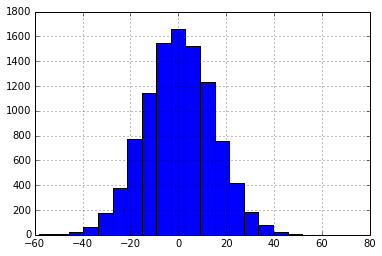
\includegraphics[width=0.6\textwidth]{diff1.png}
\end{center}

Some sample outputs of the simulation might be as follows: for \verb|numPaths = 100|, one run looks like:
\begin{center}
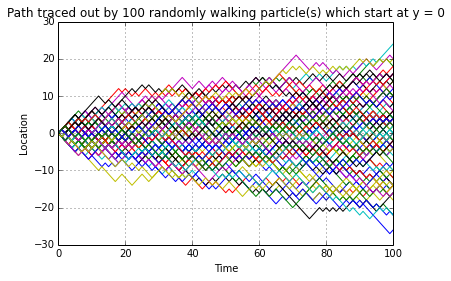
\includegraphics[width=0.6\textwidth]{diff1b.png}
\end{center}

From this, and from trying other iterations with different numbers of particles if necessary, we can see that the paths at $t = 100$ are clustered mostly around the center and thin out as you go further from $0$, which is the normal distribution drawn above.
\item As you increase the number of particles, the simulation result looks more and more continuous (less jagged edges), and it looks like a normal distribution, as shown in the solution for the first question in this section.
\item The particle is most likely to still be at 0 (the mean of the distribution is 0), no matter how many hours later or how long each step is. The means as reported from the simulations should all be close to 0. (Some error due to simulation.)
\item The relationship is that the standard deviation scales as the square root of the time: $\sqrt{\langle r^2 \rangle} \sim \sqrt{t}$, where $\langle r^2 \rangle$ is the variance, which scales as $t$. So, if the number of time steps is multiplied by $M$, the standard deviation is multiplied by $\sqrt{M}$.
\item The so-called Mendelians and biometricians disagreed because Mendelian characteristics seemed to be discrete and discontinuous, such as colors of peas or whether they were shriveled or not. On the other other hand, biometricians pointed towards continuous features, such as height. The convergence of discrete features to a continuous distribution bridged this gap and ended the argument, since in this context the ``many-variable limit'' is known as ``polygenic inheritance'', leading to a continuous distribution of traits that is further blurred by environmental factors. As one adds more particles to the simulation (i.e. more genes), the distribution converges better to the normal distribution (i.e. traits are more continuous).
\item This is an example of 1-d diffusion, so we have $\langle r^2 \rangle = 2Dt$, or

\begin{align*}
r_{rms} &= \sqrt{2Dt}\\
t &= \frac{r_{rms}^2}{2D} = \frac{0.01^2}{2(6.9\times 10^{-11})}
\end{align*}

and plugging in we have \fbox{$t \approx 8.4 \textrm{ days}$} on average. This makes sense given the result of the third simulation, since, as you can see in the figure below, for a long time period diffusion does not move the particle very far. Diffusion must not be the only effect taking place to move hemoglobin in blood, because otherwise our bodies would not function correctly (if it took 8 days to move 1 cm).

\begin{center}
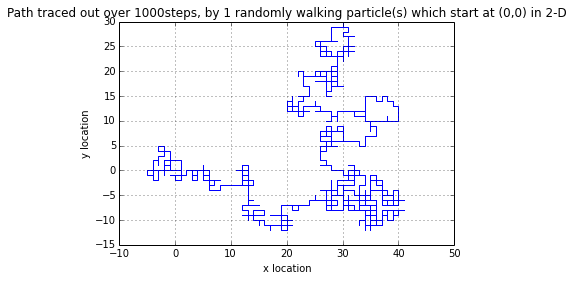
\includegraphics[width=0.6\textwidth]{diff2.png}
\end{center}
\end{enumerate}

\subsection{An interesting additional problem}
\begin{enumerate}
\item First, let us estimate the number of words in \textit{War and Peace}, which is notoriously long. On average there are around 500 words which can fit onto a page, and the novel is on the order of 1200 pages, giving us 600000 words. Each English word has around 4.5 characters, and with spaces (0.5 space to each word on each side of a space), we can call it 5 characters per word, giving us 3 million characters. Each character in ASCII encoding takes up 1 byte, so the uncompressed size is around \fbox{3 million bytes}, or around \fbox{3 megabytes}.\\

Can we do better? What would the file under compression in both the naive and typical limits look like? Consider the entropy of a random variable $X$ which can take on discrete values $\{x_1, x_2, \ldots, x_n\}$ and probability mass function $P(X_i) = p_i$. Then the Shannon entropy is:

\begin{equation*}
H = -\sum_i p_i \log_2 p_i
\end{equation*}

If we very naively take the case of English, ignoring all things such as patterns of words and word frequencies, we can model the language as a random variable $X$ which takes on one of 26 values (each letter of the alphabet) with equal probability $1/26$. Then, the Shannon entropy $H_n$ ($n$ for naive) is:

\begin{equation*}
H_n = -26\left(\frac{1}{26}\right)\log_2\left(\frac{1}{26}\right) = \log_2 26 \approx 4.7 \textrm{ bits per letter}
\end{equation*}

So, naively we know the worst case (lower bound) on compression limit is around \fbox{$4.7/8 \approx 60\%$} of the original. Of course, we know we can do much better than this, since the letters in English are not all equally likely to be used. Can we do any worse? Probably not - you can prove that the Shannon entropy is maximized for a given number of letters in an alphabet $n$ if the probabilities $p_i$ are all the same. Consider the following argument:

\begin{align*}
H &= -\sum_i p(X_i) \log_2 p(X_i)\\
&= \E\log_2\left(\frac{1}{p(X_i)}\right) \leq \log_2\left(\E\left(\frac{1}{p(X_i)}\right)\right) \hspace{3em}\textrm{ (by Jensen's inequality)}\\
\end{align*}

where

\begin{align*}
\log_2\left(\E\left(\frac{1}{p(X_i)}\right)\right)  &= \log_2 \sum_i p(X_i) \frac{1}{p(X_i)} = \log_2\sum_i 1 = \log |X| = \log_2 26
\end{align*}

so we see that $H \leq \log_2 26$ for the English language, with equality if all the $p_i$'s are equal to each other and to $1/26$. 

An interesting note: Shannon conducted some experiments which showed that the average entropy for the English language in daily usage is actually 1.0 to 1.1 bits, so a perfect compression of \textit{War and Peace} would actually be 1/8 the size of 3 megabytes, or around 0.375 megabytes. I looked up the actual sizes on Project Gutenberg, and the uncompressed text is 3.1 MB, and the compressed file is around 1.3 MB. So, we are dead on with our uncompressed approximation, and the compressed version falls within our bounds of 0.375 MB and 4.7 MB. 
\end{enumerate}


\section{Remarks}
The entirety of this simulation library, problem set (\LaTeX included), and writeup will be uploaded to \url{https://github.com/bksim/spu20-simulations}. I want to thank Professors Logan McCarty and Andrew Berry, as well as Cristina Popa, for a fruitful and enjoyable semester dedicated to pondering the question for which this class is named. I can only hope to learn more in the future about such a strange and difficult question.

\section{References}
\begin{enumerate}
\item McCarty, Logan and Berry, Andrew. \textbf{2014}, Science of the Physical Universe 20, Course Notes. Cambridge, MA.
\item \textbf{2014}, Project Gutenberg. \url{https://www.gutenberg.org/}.
\item UC Berkeley. Table of diffusion constants. \textbf{2003}, UC Berkeley. \url{http://www.cchem.berkeley.edu/chem130a/past/2003Fall/g03hw/hw9.pdf}
\end{enumerate}
\end{document}